\begin{vbframe}{Linear SVM -- Functionality}

\maketag{SUPERVISED} \maketag{CLASSIFICATION} \maketag{PARAMETRIC} 
\maketag{BLACK-BOX} 
\medskip

\highlight{General idea}

\begin{itemize}
  \item Find linear decision boundary (\textbf{separating hyperplane}) that 
  best separates classes
  \begin{itemize}
    \item \textbf{Hard-margin} SVM: maximize distance (\textbf{margin} 
    $\gamma$ > 0) to closest members (\textbf{support vectors, SV}) on each 
    side of decision boundary
    \item \textbf{Soft-margin} SVM: relax separation to allowing margin 
    violations $\rightarrow$ maximize margin while minimizing violations
  \end{itemize}
  \item 3 types of training points
  \begin{itemize}
    \item \textbf{non-SVs} with no impact on decision boundary
    \item \textbf{SVs} located exactly on decision boundary
    \item \textbf{margin violators}
  \end{itemize}
\end{itemize}

\medskip

\highlight{Hypothesis space} ~~
$\Hspace = \left\{f: \Xspace \to \R ~|~\fx = \thetab^\top \xv + \theta_0\right\}$
 ~~ \textcolor{blue}{separater intercept notwendig?}

\framebreak

\medskip
\footnotesize
\begin{minipage}{0.6\textwidth}
  \centering
  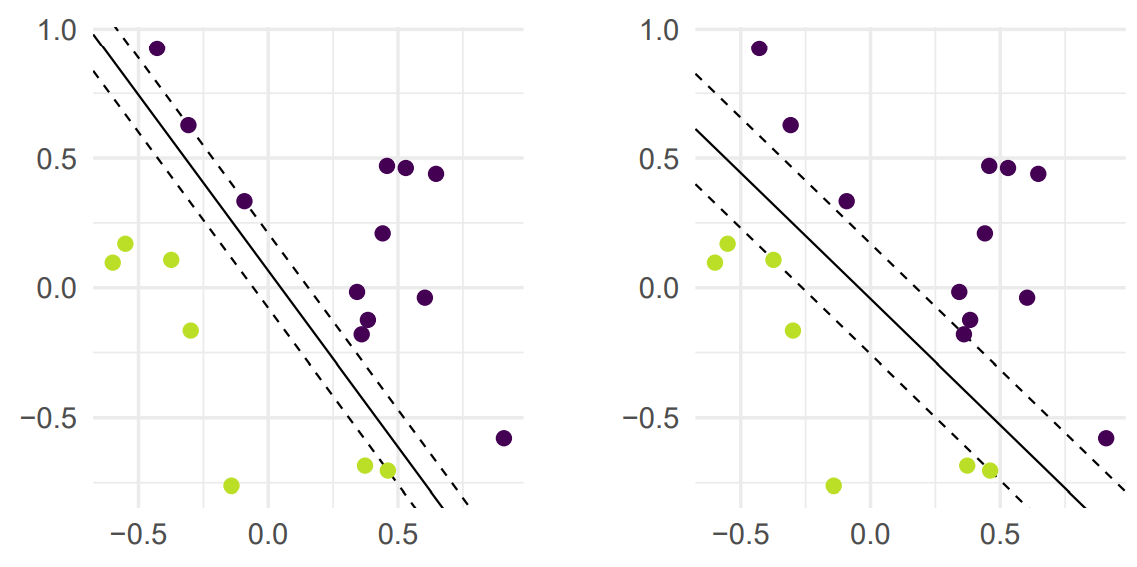
\includegraphics[width=0.9\textwidth]{figure/svm_motivation_hard_margin.png}
  \\
  \tiny{Hard-margin SVM: margin is maximized by boundary on the right}
\end{minipage}
\hfill
\begin{minipage}{0.3\textwidth}
  \centering
    %https://docs.google.com/presentation/d/1g7q1hbTNmQeuRWQIM8SF9l6iKWmJyuhyhm3s9QjA0jM/edit?usp=sharing
%from FCIM 2020/Linear SVM /slides-3-soft-margin (last plot, page8)
  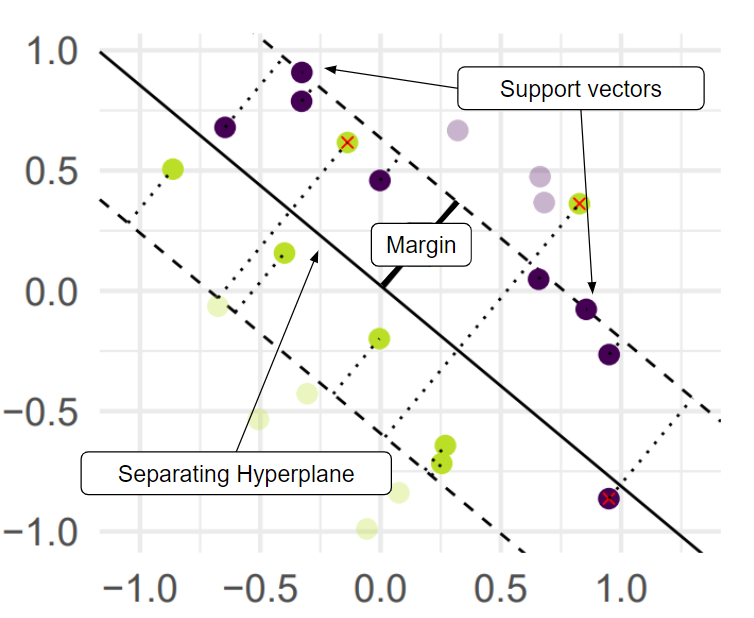
\includegraphics[width=1.1\textwidth]{figure/svm_wording.png} \\
  \tiny{Soft-margin SVM with margin violations}
\end{minipage}

\medskip

\highlight{Dual problem} ~~ %lecture_cim2\2020\08-linear-svm\slides-3-soft-margin-svm.Rnw
\begin{eqnarray*}
    & \max\limits_{\alphav \in \R^n} & \dualobj \\
    & \text{s.t. } & 0 \le \alpha_i \le C ~~ \forall i \in \nset ~~ (C = \infty
    \text{ for hard-margin SVM)}, \\
    & \quad & \sum_{i=1}^n \alpha_i \yi = 0
\end{eqnarray*}

\framebreak

\highlight{Empirical risk}

Soft-margin SVM also interpretable as \textbf{L2-regularized ERM}: 

\begin{minipage}[c]{0.58\textwidth}
  $$ \frac{1}{2} \|\thetab\|^2 + C \sumin \Lxyi$$ 
  with  
  \begin{itemize}
    \item $\|\thetab\| = 1 / \gamma$,\\
    \item $C > 0$: penalization for missclassified data points
    \item $\Lyf = \max(1-yf, 0)$: \textbf{hinge} loss \\
    $\rightarrow$ other loss functions applicable (e.g., \textbf{Huber} loss)
  \end{itemize}
\end{minipage}
\begin{minipage}[c]{0.4\textwidth}
  \centering
  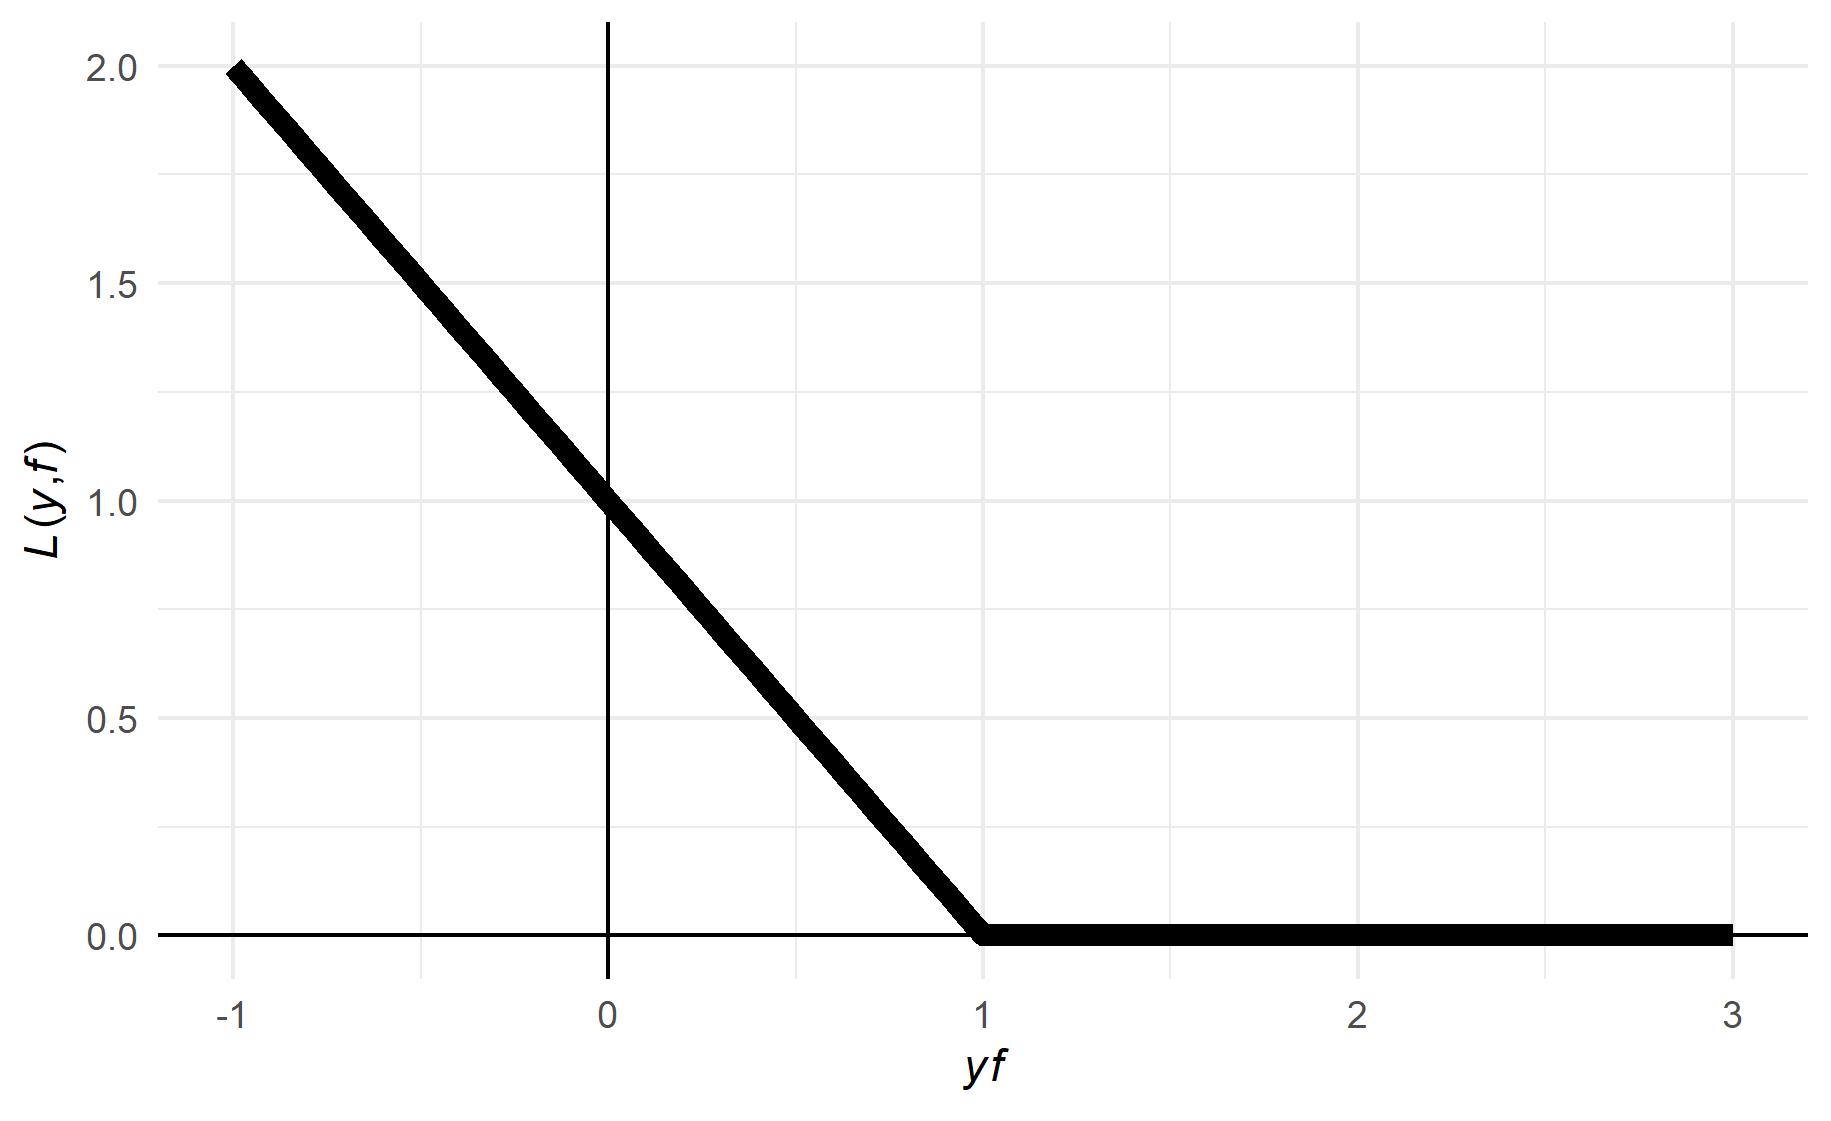
\includegraphics[height=0.4\textwidth, keepaspectratio=true]{
  figure/plot-hinge-loss.png}
\end{minipage}

%$$ \frac{1}{2} \|\thetab\|^2 + C \sumin \Lxyi ;\; \Lyf = \max(1-yf, 0),$$ 
% with  $\|\thetab\| = 1 / \gamma$, $C$ as cost parameter for margin violation and $\Lyf$ as the hinge loss.

% \begin{figure}
%   \begin{center}
%   %rsrc/plot-hinge-loss.R
%     
%   \end{center}
% \end{figure}


\vspace{1cm}

\highlight{Optimization} ~~
\textbf{Non-differentiable} problem $\rightarrow$ mostly \textbf{sub-gradient} 
methods 
%%%%%%% FIX ME from FCIM 
% As the problem is \textbf{not differentiable}, there are the following solutions: 
% \begin{enumerate}
% \item Use a smoothed loss (squared hinge, huber), then do gradient descent.\\
%   NB: Will not  create a sparse SVM if we do not add extra tricks.
% \item Use \textbf{subgradient} methods.
% \item Do stochastic subgradient descent.\\
%   Pegasos: Primal Estimated sub-GrAdient SOlver for SVM.
% \end{enumerate}

\medskip

\highlight{Hyperparameters} ~~ Cost parameter \textbf{$C$}

%https://www.ijcaonline.org/research/volume128/number3/abdiansah-2015-ijca-906480.pdf
% \highlight{Runtime behavior} ~~ \textcolor{blue}{$\mathcal{O}(n^3)$ for $n$ observations} %$\mathcal{O}(n^2 \cdot p + n^3)$ for $n$ observations and $p$ features

\end{vbframe}

% ------------------------------------------------------------------------------

\begin{frame}{Linear SVM -- Pro's \& Con's}

\footnotesize


\begin{columns}[onlytextwidth]
  \begin{column}{0.5\textwidth}
    \highlight{Advantages}
    \footnotesize
    \begin{itemize}
      \positem high \textbf{accuaracy}
      \positem often \textbf{sparse} solution
      \positem robust against overfitting (\textbf{regularized}); especially in high-dimensional space
      \positem \textbf{stable} solutions, as the non-SV do not influence the separating hyperplane
      %\positem \textbf{memory efficient} (only use non-SVs)
    \end{itemize}
  \end{column}

  \begin{column}{0.5\textwidth}
    \highlight{Disadvantages}
    \footnotesize
    \begin{itemize}
      \negitem \textbf{costly implementation}; long training times
      \negitem does not scale well to \textbf{larger data sets} \textcolor{blue}{\textbf{??}}
      \negitem only \textbf{linear separation} $\rightarrow$ possible with non-linear SVMs which are explained in the following slides.
      \negitem poor \textbf{interpretability}
    \end{itemize}
  \end{column}
\end{columns}

\vfill

\small

\conclbox{Very accurate solution for high-dimensional data that is linearly separable}

\end{frame}

% ------------------------------------------------------------------------------

\begin{frame}{Linear SVM -- Practical hints}

\footnotesize

  \highlight{Preprocessing} \\
  Features must be rescaled before applying SVMs.
  
  \medskip
  
  \highlight{Tuning} \\
  The cost parameter $C$ must be tuned, as it has a strong influence on the resulting separating hyperplane. 

  \medskip

  \highlight{Implementation} 
  \begin{itemize}
    \item \textbf{R:} \texttt{mlr3} learners \texttt{LearnerClassifSVM} / 
    \texttt{LearnerRegrSVM}, calling \texttt{svm()} from \texttt{libsvm}
    \item \textbf{Python:} \texttt{sklearn.svm.SVC} from package \texttt{scikit-learn} / package \texttt{libSVM}
  \end{itemize}

\end{frame}
